% !TEX root = ../main.tex

This high severity attack took place in April, 2018 due to a well known and common issue in many programming languages called \textit{integer overflow} \footnote{\url{https://en.wikipedia.org/wiki/Integer\_overflow}}. It termed as \textbf{batchOverflow} or \textbf{proxyOverflow} and some exchanges (such as OKEx\footnote{\url{https://okex.com}}, Poloniex\footnote{\url{https://poloniex.com/}}, HitBTC\footnote{\url{https://hitbtc.com/}} and Huobi Pro\footnote{\url{https://www.huobi.com/en-us/>}}) suspended deposits and withdrawals of ALL tokens, especially for Beauty Ecosystem Coin (BEC\footnote{\url{https://etherscan.io/address/0xc5d105e63711398af9bbff092d4b6769c82f793d}}) that was targeted by this exploit.

\subsubsection{Attack analysis}
In this attack, malicious person was able to run a transaction\footnote{\url{https://etherscan.io/tx/0xad89ff16fd1ebe3a0a7cf4ed282302c06626c1af33221ebe0d3a470aba4a660f}} and transfer two extremely large amount of BEC tokens to two Ethereum addresses. Although BEC developers had considered most of the security measurements, only line 257 of the code (see Figure~\ref{fig:bec}) was vulnerable against this classic integer overflow attack\cite{PeckShield01}. The attacker was able to pass a combination of input values that generate large results than the maximum value of \texttt{uint256} data type can hold. This caused integer overflow and only the least significant bits have been retained. In other words, the \texttt{uint256} variable reached to its maximum value that can be held and it \textit{wraps around\footnote{\url{https://en.wikipedia.org/wiki/Integer\_overflow}}} by starting from 0. For example, an \texttt{uint8} (8-bit unsigned integer) can represent maximum value of $2^8-1=255 (\mathtt{0xff})$. Multiplying \texttt{0x02} by \texttt{0x80} causes integer overflow and produces \texttt{0x00} as the result ($\mathtt{0x02} \times \mathtt{0x80} = \mathtt{0x100} \rightarrow \mathtt{0x00}$). We can achieve the same result by adding \texttt{0x01} to \texttt{0xff} ($\mathtt{0x01} + \mathtt{0xff} = \mathtt{0x100} \rightarrow \mathtt{0x00}$). So, In BEC case, the attacker passed two addresses (\texttt{cnt = \_receivers.lengh = 0x02}) and a large value (\texttt{\_value = 0x8000000000000000000000000000000000000000000000000000000000000000} (63 0's)) to \texttt{batchTransfer()} function. Because of wrap around, the result of \texttt{amount} variable in line 257 was calculated as \texttt{0x00} and bypassed sanity checks in line 259 (see Figure~\ref{fig:bec}). Hence, line 264 transferred the specified \texttt{\_value} to those two addresses. The transferred amount was even larger than the initial supply of the token-- that was \texttt{7000000000000000000000000000} (27 0's) tokens, hence allowing the attacker to take control of token finance and manipulate its price.

\begin{figure}[t]
	\centering
	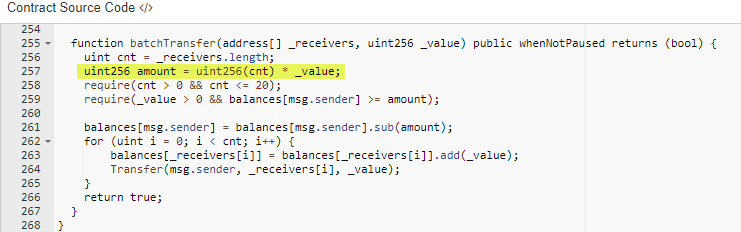
\includegraphics[width=0.9\linewidth]{figures/img03.png}
	\caption{Vulnerable code in BEC token, \texttt{batchTransfer()} function.}
	\label{fig:bec}
\end{figure}

Smart(SMT\footnote{\url{https://etherscan.io/address/0x55f93985431fc9304077687a35a1ba103dc1e081\#code}}) and Mesh(MESH\footnote{\url{https://etherscan.io/address/0x3ac6cb00f5a44712022a51fbace4c7497f56ee31\#code}}) were the next victims of this exploit. The attackers were able to transfer\footnote{\url{https://etherscan.io/tx/0x1abab4c8db9a30e703114528e31dee129a3a758f7f8abc3b6494aad3d304e43f}} \texttt{0x8fffffffffffffffffffffffffffffffffffffffffffffffffffffffffffffff} (63 f’s) tokens to one address \footnote{\url{https://etherscan.io/token/0x55f93985431fc9304077687a35a1ba103dc1e081?a=0xdf31a499a5a8358b74564f1e2214b31bb34eb46f}} and \texttt{0x70000000000000000000000000000000000000000000000000000000000-
00001} (62 0's) as huge fee to the transaction initiator\footnote{\url{https://etherscan.io/address/0xd6a09bdb29e1eafa92a30373c44b09e2e2e0651e}}.

\begin{figure}[t]
	\centering
	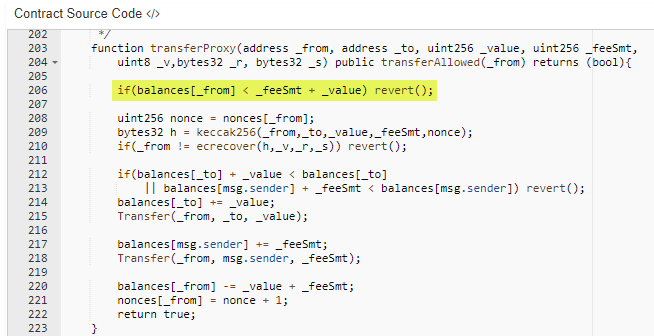
\includegraphics[width=1.0\linewidth]{figures/img04.png}
	\caption{Vulnerable code in SMT token. Passing two large values to the \texttt{transferProxy()} function bypasses sanity check in line 206 and makes the attack possible.}
	\label{fig:smt}	
\end{figure}

They executed  \texttt{transferProxy()} function (see Figure~\ref{fig:smt}) which was designed for transferring tokens on behalf of someone else by taking a fee. Line 206 of this ERC20 token was vulnerable and sum of \texttt{\_feeSmt} and \texttt{\_value} produced zero. Consequently, this bypassed the sanity check and allowed execution of the reset of the code that resulted in this attack. In addition to BEC, SMT and MESH tokens, the following ERC20 tokens have been identified as overflow-affected\cite{PeckShield02}:

\begin{enumerate}
	\item UGToken\footnote{\url{https://etherscan.io/address/0x43ee79e379e7b78d871100ed696e803e7893b644\#code}}
	\item SMART\footnote{\url{https://etherscan.io/address/0x60be37dacb94748a12208a7ff298f6112365e31f\#code}}
	\item MTC\footnote{\url{https://etherscan.io/address/0x8febf7551eea6ce499f96537ae0e2075c5a7301a\#code}}
	\item First\footnote{\url{https://etherscan.io/address/0x9e88770da20ebea0df87ad874c2f5cf8ab92f605\#code}}
	\item GGoken\footnote{\url{https://etherscan.io/address/0xf20b76ed9d5467fdcdc1444455e303257d2827c7\#code}}
	\item CNYToken\footnote{\url{https://etherscan.io/address/0x041b3eb05560ba2670def3cc5eec2aeef8e5d14b\#code}}
	\item CNYTokenPLus\footnote{\url{https://etherscan.io/address/0xfbb7b2295ab9f987a9f7bd5ba6c9de8ee762deb8\#code}}
	\item MESH\footnote{\url{https://etherscan.io/address/0x3ac6cb00f5a44712022a51fbace4c7497f56ee31\#code}}
\end{enumerate}

\subsubsection{Reproducing the attack}
To check feasibility of this attack in the current version of Solidity\footnote{An object-oriented programming language for writing smart contracts on the Ethereum blockchain} compiler (0.5.10 as July 2019), a demo smart contract (called \texttt{multiplyDemo} as shown in Figure~\ref{fig:ovfdemo}) is created and used to test overflow issue. As it can be seen, the \texttt{a\_multiply\_b()} function multiplies \texttt{a} and \texttt{b} to exceed maximum capacity of \texttt{uint256} data type and set \texttt{c} variable to 0 (due to \textit{wraps around}). We have initially set \texttt{c=0x3} to check its result before and after multiplication performed by \texttt{a\_multiply\_b()} function. 
\begin{figure}[t]
	\centering
	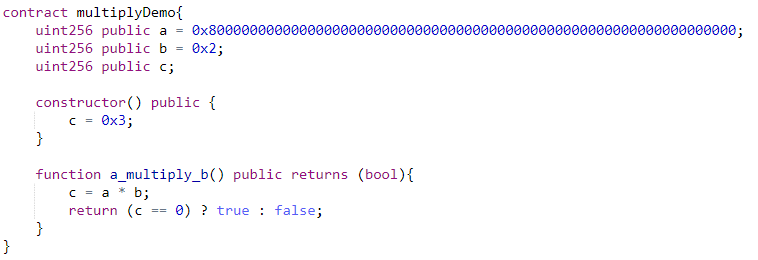
\includegraphics[width=1.0\linewidth]{figures/img05.png}
	\caption{Integer overflow demonstration in multiplication of \texttt{uint256} variables}
	\label{fig:ovfdemo}
\end{figure}

Running this code on the RemixIDE\footnote{Online programming tool for developing smart contracts on the Ethereum blockchain. It supports Solidity and Vyper programming languages. \url{https://remix.ethereum.org/}} returns \texttt{true} (since \texttt{c=0}). Transaction log also shows that Ethereum has executed \texttt{a\_multiply\_b()} function in unchecked context\footnote{In an unchecked context, arithmetic overflow is ignored and the result is truncated by discarding any high-order bits that don't fit in the destination type.} and logged successful status by returning \texttt{true} as output of the function (see figure~\ref{fig:ovftran}).

\begin{figure}[t]
	\centering
	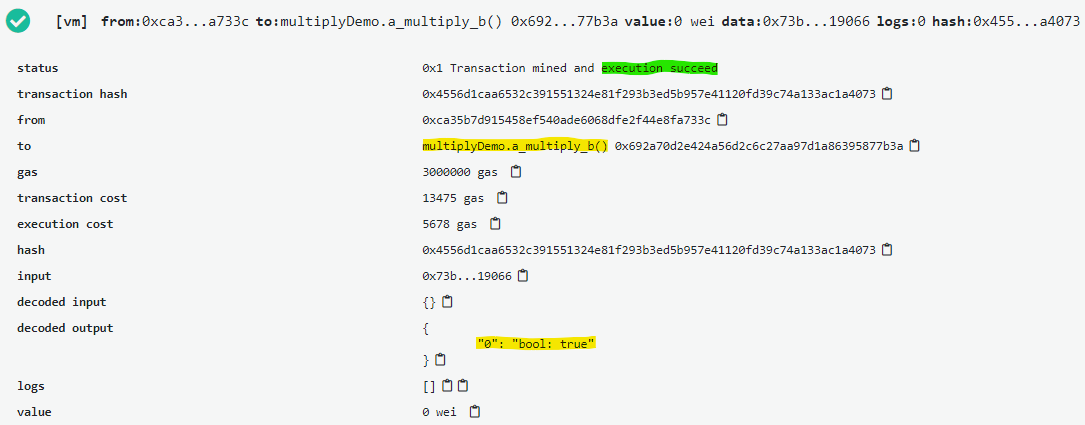
\includegraphics[width=1.0\linewidth]{figures/img06.png}
	\caption{Multiplication of \texttt{a} and \texttt{b} by \texttt{a\_multiply\_b()} function causes \texttt{uint256} overflow. It returns \texttt{true} since the result is 0. It implies \textit{wraps around} in unchecked context of Ethereum.}
	\label{fig:ovftran}
\end{figure}

The same result can be seen from RemixIDE interface (see Figure~\ref{fig:ovfmul}). On the left, \texttt{c} is 3 before execution of \texttt{a\_multiply\_b()} function and on the right, it is 0 after that.
\begin{figure}[t]
	\centering
	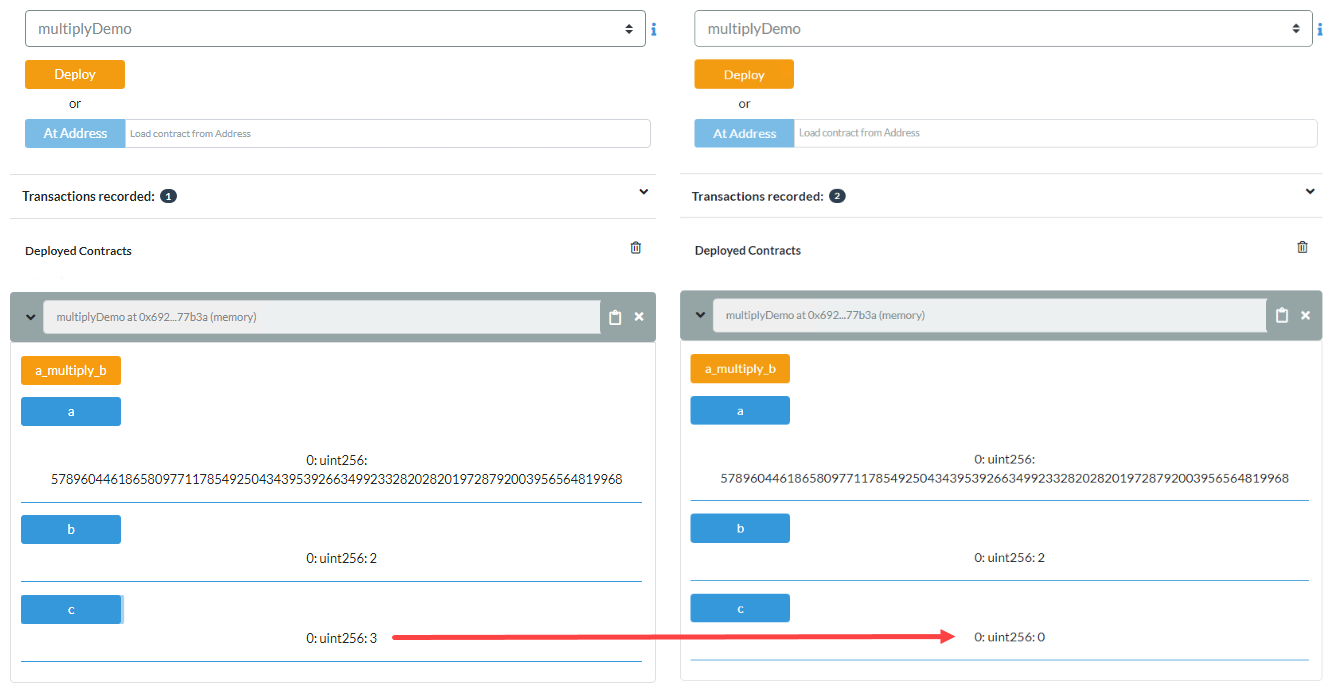
\includegraphics[width=1.0\linewidth]{figures/img07.png}
	\caption{Overflow issue in multiplication. On the left, before execution of \texttt{a\_multiply\_b()} and on the right, after that. \texttt{c} variable is set to zero due to \textit{wraps around}.}
	\label{fig:ovfmul}
\end{figure}

By default, integer overflow does not throw a runtime exception in Ethereum. This is by design and we can get the same overflow issue in the summation of two \texttt{uint256} variables. To reproduce the issue, we created another demo smart contract with \texttt{a\_plus\_b()} function that adds two variables. In this case the result (\texttt{c} variable) sets to 0 due to wraps around (see Figures~\ref{fig:ovfsum} and ~\ref{fig:ovftran2}).

\begin{figure}[t]
	\centering
	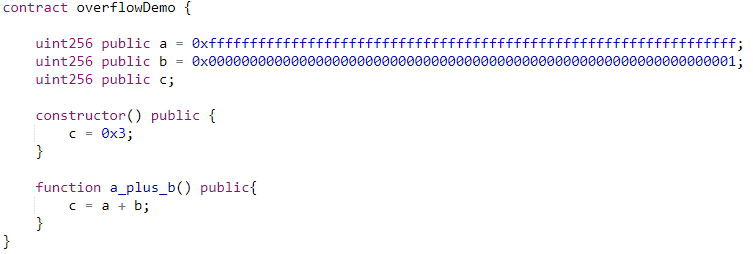
\includegraphics[width=0.9\linewidth]{figures/img08.png}
	\caption{Sample code to demonstrate integer overflow issue in summation of \texttt{uint256} variables}
	\label{fig:ovfsum}
\end{figure}

\begin{figure}[t]
	\centering
	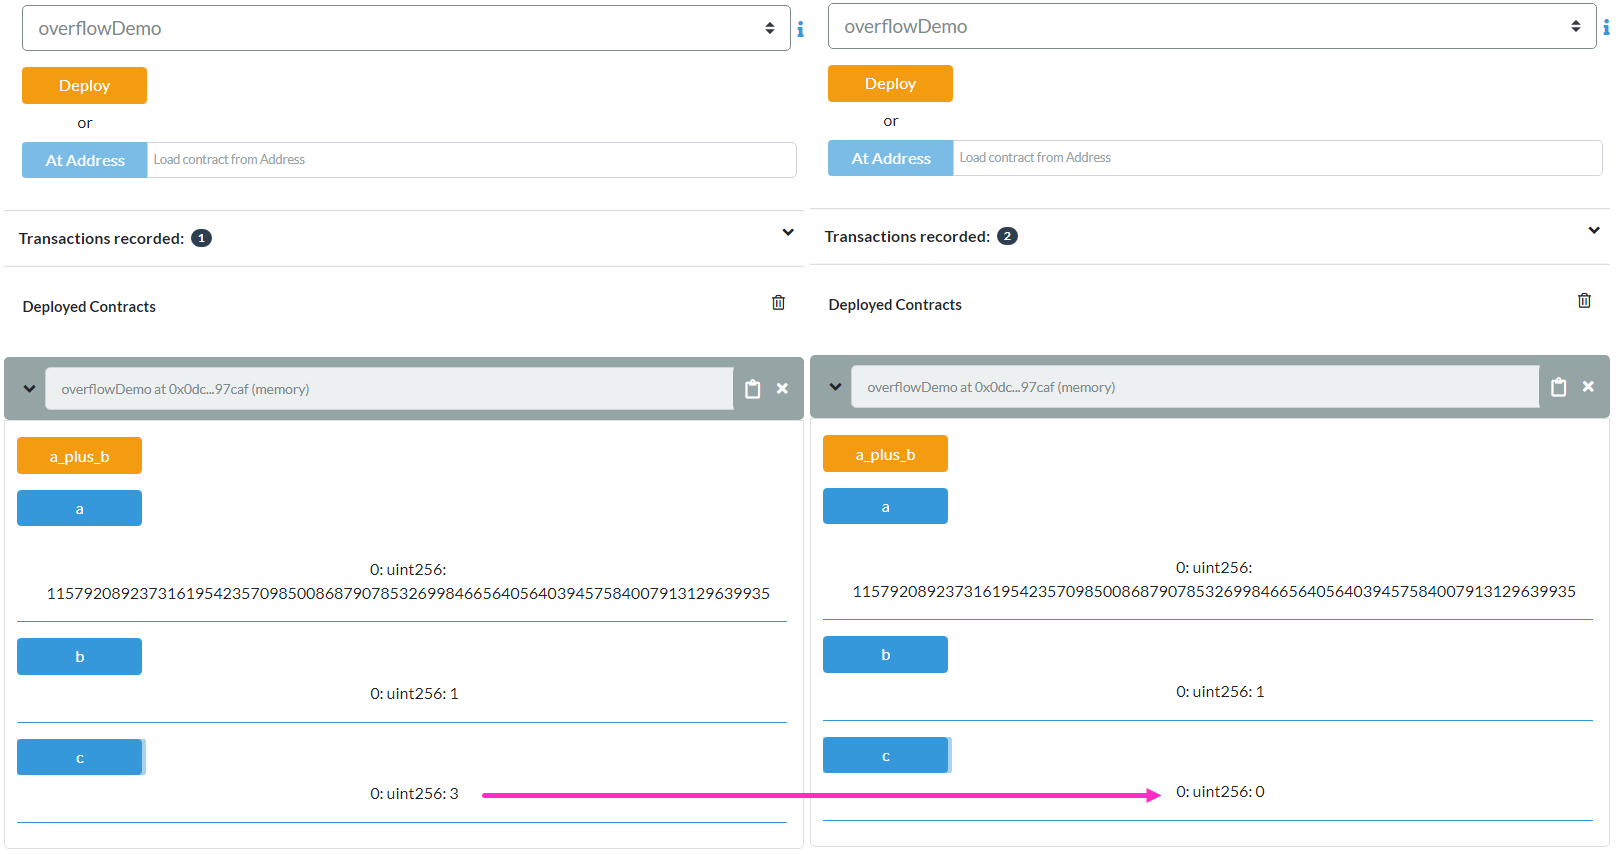
\includegraphics[width=1.0\linewidth]{figures/img09.png}
	\caption{Possibility of integer overflow in summation. On the left, before execution of \texttt{a\_plus\_b()} and on the right, after that. \texttt{c} variable is set to zero due to \textit{wraps around}.}
	\label{fig:ovftran2}
\end{figure}

\subsubsection{Attack mitigation}
As analyzed in the previous section, the arithmetic result of numeric values outside of the representable range will lead to wrap around and sets the result to 0. Although this behaviour is expected in Ethereum, it causes security problems as explained in CVE-2018–10299\footnote{\url{https://nvd.nist.gov/vuln/detail/CVE-2018-10299}} and CVE-2018-10376\footnote{\url{https://nvd.nist.gov/vuln/detail/CVE-2018-10376}}. To address this issue, it is recommended to use \texttt{SafeMath} library\footnote{\url{https://github.com/OpenZeppelin/zeppelin-solidity/blob/master/contracts/math/SafeMath.sol}} when performing any arithmetic calculation. This library is offered by OpenZeppelin\footnote{\url{https://github.com/OpenZeppelin/openzeppelin-solidity}} and has become industry standard for catching overflows. Moreover, auditing before launching the code could also prevent such human errors and help to be in compliance with the best practices. We used \texttt{SafeMath} library and re-implemented vulnerable functions to examine its effectiveness (see Figures~\ref{fig:addsafe} and ~\ref{fig:ovfaddsafe}).

\begin{figure}[t]
	\centering
	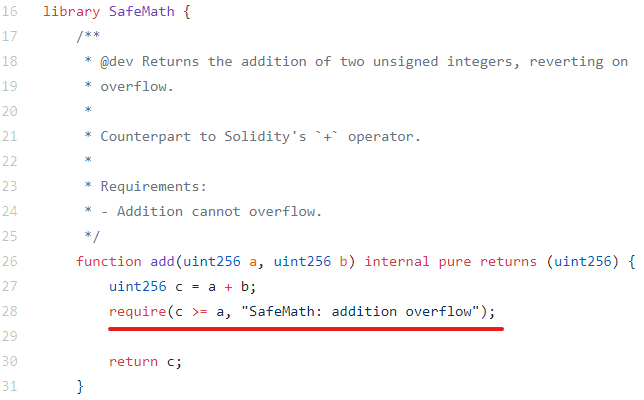
\includegraphics[width=0.7\linewidth]{figures/img12.png}
	\caption{\texttt{Add} function of \texttt{SafeMath} library checks for overflow and raises an error in line 28. The \texttt{require()} function simply checks for the result to be greater than input (\texttt{a}) and throws an exception if the condition is not met. It returns an error message that can be retreived from the exception handler.}
	\label{fig:addsafe}
\end{figure}

\begin{figure}[t]
	\centering
	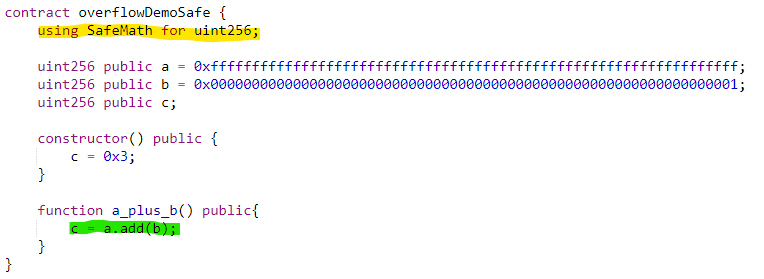
\includegraphics[width=0.75\linewidth]{figures/img10.png}
	\caption{Using \texttt{SafeMath} library to prevent overflow attack.}
	\label{fig:ovfaddsafe}
\end{figure}
%%%%%%The Following sentence is not clear! %%%%%%%%
By adding "\texttt{using}"\footnote{\url{https://solidity.readthedocs.io/en/v0.5.10/contracts.html?highlight=Library\#libraries}} keyword to \texttt{a\_plus\_b()} function, we could give any \texttt{uint256} within the \texttt{a\_plus\_b()} function the libraries functions and pass the \texttt{uint256} as the first parameter. As highlighted, \texttt{a.add(b)} calls \texttt{add(uint256 a, uint256 b)} from \texttt{SafeMath} library and passes \texttt{b} as input variable. The \texttt{add} function in \texttt{SafeMath} checks the result and raises an error message in case of integer overflow (see Figure~\ref{fig:ovfaddexcep}). Throwing an exception will undo all state changes and stop execution of the transaction. Therefore, it mitigates the attack effectively.

\begin{figure}[t]
	\centering
	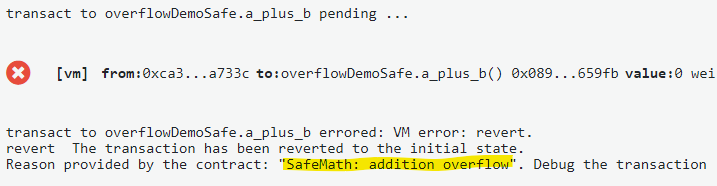
\includegraphics[width=0.7\linewidth]{figures/img11.png}
	\caption{Reverted transaction by \texttt{SafeMath} due to overflow check.}
	\label{fig:ovfaddexcep}
\end{figure}

